\documentclass{beamer}
\usetheme{Warsaw}

\usepackage[utf8]{inputenc}
\usepackage{fancybox}
\usepackage{multimedia} 
\usepackage{subfig}
\usepackage{amsmath}
\usepackage{hyperref}
\usepackage[all]{xy}
\usepackage{algorithm}
%\usepackage{arevmath}     % For math symbols
\usepackage[noend]{algpseudocode}
\setbeamertemplate{footline}[frame number]

\begin{document}



\title[Stochastik] % (optional, only for long titles)
{Stochastik für Informatiker
\\
\includegraphics[scale=0.5]{img/craps}
}
\subtitle{}
\author[Dr. Johannes Riesterer] % (optional, for multiple authors)
{Dr.  rer. nat. Johannes Riesterer}

\date[KPT 2004] % (optional)
{}

\subject{Stochastik}





\begin{frame}
    \frametitle{Angewandte Mathematik}
\framesubtitle{Lebesgue Integral}
\begin{block}{Quader und lineare Abbildungen}
Seien $U$ und $V$ offene Teilmengen des $\mathbb{R}^n$, $T': U \to V$ ein lineare Abbildung und  $Q \in \mathbb{I}(n)$ ein Quader.
Dann gilt:
 $$ \text{vol}  (T'(Q))   =  \det (T') \cdot   \text{vol}(Q) \; .$$
\end{block}
 \end{frame}

\begin{frame}
    \frametitle{Angewandte Mathematik}
\framesubtitle{Beweis}
Für Vektoren $a_1, \cdots a_n$ im $\mathbb{R}^n$ heißt die Menge 
$$ P(a_1, \cdots,  a_n) := \biggl \{  x = \sum_{k=1}^n t_k a_k  \; | \; t_1, \cdots , t_n \in [0,1]  \biggr \}$$
Parallelotop.
\begin{figure}[H]
      \centering
    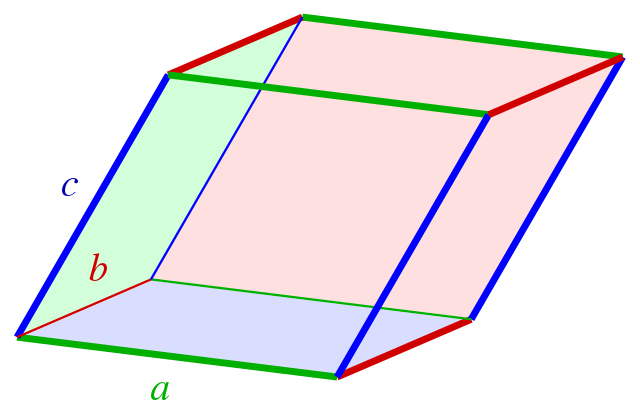
\includegraphics[width=0.6 \textwidth]{img/640px-Parallelepiped-0}    
\end{figure}
 \end{frame}

\begin{frame}
    \frametitle{Angewandte Mathematik}
\framesubtitle{Beweis}

Es gilt  $$  \text{vol} \bigr( P(a_1, \cdots, a_n) \bigr) =  | det (a_1, \cdots, a_n) |   \; .$$

\href{https://www.math.uchicago.edu/~may/VIGRE/VIGRE2007/REUPapers/FINALAPP/Peng.pdf}{Ausfürlicher Beweis}
 \end{frame}



\begin{frame}
    \frametitle{Angewandte Mathematik}
\framesubtitle{Lebesgue Integral}
\begin{block}{Diffeomorphismus}
Seien $U$ und $V$ offene Teilmengen des $\mathbb{R}^n$. Eine Abbildung  $T: U \to V$ heißt Diffeomorphismus, wenn eine  Umkehrfunktion $T^{-1}: V  \to U$ existiert, also $T^{-1} (T (u)) = u$ gilt für alle $u \in U$, die ebenfalls differenzierbar ist.
\end{block}

\begin{block}{}
Für eine invertierbare Matrix $A$ ist $T(x):= Ax$ ein Diffeomorphismus.
\end{block}
 \end{frame}


\begin{frame}
    \frametitle{Angewandte Mathematik}
\framesubtitle{Lebesgue Integral}
\begin{block}{Transformationssatz}
Seien $U$ und $V$ offene Teilmengen des $\mathbb{R}^n$, $T: U \to V$ ein Diffeomorphismus und $f: V \to \mathbb{R}$ eine integrierbare Funktion. Dann gilt:
$$ \int_V  f(y)  d \mu = \int_U f(T (x))  \cdot | \det(T' (x)) | d \mu   \; .$$
\end{block}
 \end{frame}

\begin{frame}
    \frametitle{Angewandte Mathematik}
\framesubtitle{Beweis}
Seien $I_k \in \mathbb{I}(n)$ Quader, $J_k := T(I_k)$ und $b_k = T(c_k)$. Dann ist 
$$\sum_{k=1}^n  b_k  \text{vol}(J_k) \approx  \sum_{k=1}^n T(c_k) \cdot | \det T' (c_k)|  \text{vol}(I_k) \; .$$
Die Behauptung folgt dann (nicht trivial) durch den Übergang zu Grenzwerten mit entsprechenden Konvergenzsätzen.
 \end{frame}


\begin{frame}
    \frametitle{Angewandte Mathematik}
\framesubtitle{Lebesgue Integral}
\begin{block}{Beispiel}
Wir betrachten den Ball $B_r^3(0):= \{ x \in \mathbb{R}^3 \; | \; || x || \leq r  \}$, den Quader $I := [0,r] \times [- \pi, \pi] \times [- \frac{\pi}{2}, \frac{\pi}{2}]$ und die Abbildung
\begin{align*}
T : I \to B_1^3(0) \\
T(r, \varphi, \psi) := \begin{pmatrix} r \cos(\varphi) \cos(\psi)   \\  r \sin(\varphi) \cos(\psi) \\ r  \sin(\psi)     \end{pmatrix}
\end{align*}
\end{block}
\begin{block}{Beispiel}
$\det T'(r, \varphi, \psi) = r^2 \cos(\psi)$
\end{block}
 \end{frame}

\begin{frame}
    \frametitle{Angewandte Mathematik}
\framesubtitle{Lebesgue Integral}
\begin{align*}
\int_{B_r^3(0)} 1 d\mu = \int_{ [0,r] } \int_{ [- \pi, \pi]} \int_{[- \frac{\pi}{2}, \frac{\pi}{2}]} r^2 \cos(\psi) d \psi \; d \varphi \; dr = \frac{4} {3} \pi r^3
\end{align*}
\begin{figure}[H]
      \centering
    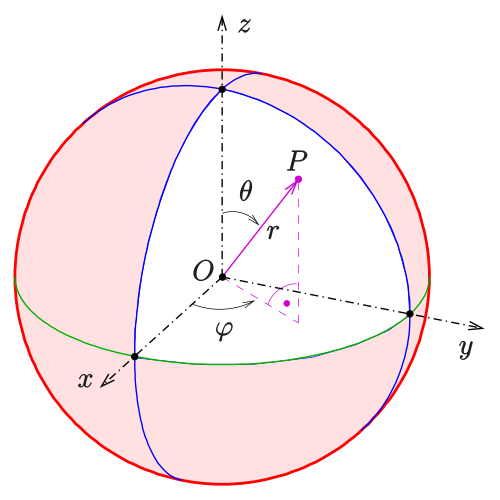
\includegraphics[width=0.4 \textwidth]{img/500px-Kugelkoord-def}    
\end{figure}
 \end{frame}



\begin{frame}
    \frametitle{Zufallsvariablen}
\framesubtitle{}

\begin{block}{Zufallsvariablen}
Sei $(\Omega, \mathcal{A}, P)$ ein Wahrscheinlichkeitsraum und $(\Omega', \mathcal{A}')$ ein Messraum. Eine Zufallsvariable ist eine messbare Abbildung 
$$X : \Omega \to \Omega'$$ 
D.h. für alle Ereignisse $A' \in  \mathcal{A}'$ ist 
$$ X^{-1} (A') \in \mathcal{A}$$
 ein Ereignis in $\mathcal{A}$. Urbilder von Ereignissen sind also Ereignisse.
\end{block}

 \end{frame}

\begin{frame}
    \frametitle{Zufallsvariablen}
\framesubtitle{}
\begin{block}{Beispiel (Münzwurf)}
$\Omega = \{\text{Kopf}, \text{Zahl} \} $, $\Omega' = \{ 0,1 \}$  mit jeweils Potenzmenge als Sigma-Algebra und 
\begin{align*}
& X (\text{Kopf} ) = 0 \\
& X (\text{Zahl} ) = 1 
\end{align*}
\end{block}

\begin{block}{Beispiel (Summe zweier Würfel)}
$\Omega = \{1,2,3,4,5,6 \} \times \{1,2,3,4,5,6 \} $, $\Omega' = \{ 2,3,4,5,6,7,8,9,10, 11, 12\}$   mit jeweils Potenzmenge als Sigma-Algebra und $X: \Omega \to \Omega'; X (a,b) := a +b$. 
\end{block}

 \end{frame}

\begin{frame}
    \frametitle{Zufallsvariablen}
\framesubtitle{}
\begin{block}{Bildmaß}
Sei $(\Omega, \mathcal{A}, P)$ ein Wahrscheinlichkeitsraum, $(\Omega', \mathcal{A}')$ ein Messraum und  $X : \Omega \to \Omega'$  Eine Zufallsvariable. 
Durch 
\begin{align*}
P_X (A') := P(X^{-1} (A'))
\end{align*}
 für $A' \in \mathcal{A}'$ wird ein Wahrscheinlichkeitsmaß auf  $(\Omega', \mathcal{A}')$ definiert. Es wird Bildmaß genannt. Anstelle von $P_X (A')$ wird auch die Schreibweise $P (X \in A'):= P_X (A')$ verwendet.
\end{block}


 \end{frame}

\begin{frame}
    \frametitle{Zufallsvariablen}
\framesubtitle{}

\begin{block}{Beispiel (Summe zweier Würfel)}
$\Omega = \{1,2,3,4,5,6 \} \times \{1,2,3,4,5,6 \} $, $\Omega' = \{ 2,3,4,5,6,7,8,9,10, 11, 12\}$ und $X: \Omega \to \Omega'; X (a,b) := a +b$. Dann ist 
$P_X(3) = P(\{(1,2), (2,1)\}) = \frac{2}{36} = \frac{1}{18}$ 
\end{block}

 \end{frame}






\begin{frame}
    \frametitle{Zufallsvariablen}
\framesubtitle{}

\begin{block}{Verteilungsfunktion}
Für eine reelle Zufallsvariable heißt 
\begin{align*} 
& F_X : \mathbb{R}^n \to [0,1] \\
& F_X (x) := P (X \leq x) := P_X (( -\infty, x )) = P(X^{-1} (-\infty, x))
\end{align*}
Verteilungsfunktion von $X$.
\end{block}
 \end{frame}

\begin{frame}
    \frametitle{Zufallsvariablen}
\framesubtitle{}

\begin{block}{Dichte}
 Eine Funktion $f:\mathbb{R}^n \to \mathbb{R}$ heißt Dichte, falls für ihr Lebesgue-Integral $\int_{\Omega} f d \mu = 1$ gilt.
\end{block}
\begin{block}{Dichte}
 Eine  Funktion $f:\Omega \to \mathbb{R}$ heißt Dichte der  Verteilungsfunktio $F_X : \Omega \to [0,1]$ falls für ihr Lebesgue-Integral $\int_{\Omega} f d \mu = 1$ ist und 
$F_X (x) = \int_{\{X \leq x \}} f d \mu$
\end{block}
 \end{frame}

\begin{frame}
    \frametitle{Zufallsvariablen}
\framesubtitle{}
\begin{block}{Beispiel}
Die Funktion $f(x) = \frac{1}{\sqrt{\pi}} e^{- x^2}$ ist eine Dichte auf $ \mathbb{R}$.
\begin{align*}
& I := \int_{0}^{\infty} e^{-x^2} \; dx\\
& I^2 =  \int_{0}^{\infty} e^{-x^2} \; dx \cdot    \int_{0}^{\infty} e^{-y^2} \; dy =    \int_{0}^{\infty} \int_{0}^{\infty} e^{-(x^2+y^2)} \; dx \;dy \\
&x=r \cos \varphi ,y=r\sin \varphi ,r^2 = x^2 + y^2  \; (\text{ da } \cos^2 + \sin^2 = 1)\\
 &\text{ \href{https://de.wikipedia.org/wiki/Polarkoordinaten\#Zylinderkoordinaten}{LINK: Polarkoordinatentransformation}} \\
& = \int_{0}^{\frac{\pi}{2}}  \int_{0}^{\infty}r \cdot e^{-r^2} \; dr \;d\varphi \\
&= \frac{\pi}{2} \int_{0}^{\infty}r \cdot e^{-r^2} \; dr \\
&= -\frac{\pi}{4} [e^{-r^2} ]_0^{\infty} = \frac{\pi}{4} \Rightarrow I = \frac{\sqrt{\pi}}{2}
\end{align*}
\end{block}
 \end{frame}


\begin{frame}
    \frametitle{Zufallsvariablen}
\framesubtitle{}
\begin{block}{Beispiel}
Analog beweist man, dass für alle  $\mu \in \mathbb{R}, \sigma > 0 $ die Funktion $ f(x):=  \frac 1{\sigma \sqrt{2\pi}}e^{- \frac {1}{2} (\frac{x- \mu}{ \sigma})^2}$  eine  Dichte auf $ \mathbb{R}$ ist.
\end{block}
\begin{figure}[htp]
      \centering
    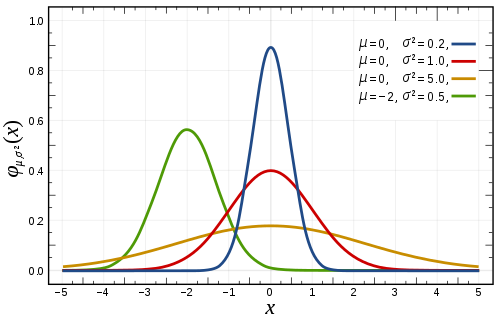
\includegraphics[width=0.76\textwidth]{img/normal}
      \caption{Quelle: Wikipedia}
\end{figure}
 \end{frame}

\begin{frame}
    \frametitle{Zufallsvariablen}
\framesubtitle{}
\begin{block}{Normalverteilung}
Eine reelle Zufallsvariable $X: \Omega \to \mathbb{R}$ heißt normalverteilt, wenn 
$F_X (x) = \int_{- \infty}^{x}  \frac 1{\sigma \sqrt{2\pi}}e^{- \frac {1}{2} (\frac{x- \mu}{ \sigma})^2}dx$ mit  $\mu \in \mathbb{R}, \sigma > 0 $ gilt. Man schreibt auch $X \sim \mathcal{N}(\mu, \sigma^2)$.
\end{block}
\begin{figure}[htp]
      \centering
    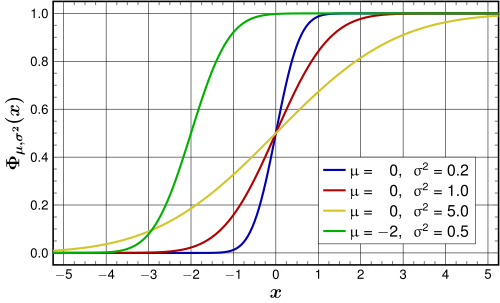
\includegraphics[width=0.76\textwidth]{img/normaldist}
      \caption{Quelle: Wikipedia}
\end{figure}
 \end{frame}



\begin{frame}
    \frametitle{Zufallsvariablen}
\framesubtitle{}
\begin{block}{Verteilung und Unabhängigkeit}
Sei $(\Omega, \mathcal{A}, P)$ ein Wahrscheinlichkeitsraum, $(R, \mathcal{B})$ ein Messraum  und
 $\{X_i\}_{i=1}^n$ ein Folge von Zufallsvariablen   $X_i :  \Omega \to R$.
Die Zufallsvariablen heißen identisch verteilt, falls
 $P_{X_i} = P_{X_j}$ für alle $i,j$  und
stochastisch unabhängig, falls
 $P_{(X_1, \cdots ,X_n)} = \prod_{i=1}^n P_{X_i}$ gilt. 
\end{block}
 \end{frame}



\begin{frame}
    \frametitle{Erwartungswert}
\framesubtitle{}
\begin{block}{Erwartungswert}
Für eine reelle integrierbare Zufallsvariableist ihr  Erwartungswert  definiert durch
$$ \mathbb{E} (X) := \int_{\Omega} X \; dP \; .$$
\end{block}
 \begin{block}{Erwartungswert}
Ist $(\Omega, \mathcal{A}, P)$ ein diskreter Wahrscheinlichkeitsraum und $X :\Omega \to \mathbb{R}$ eine reelle Zufallsvariable, so ist
$$ \mathbb{E} (X) = \sum_{\omega \in \Omega}  X(\omega) \cdot P(\omega)$$
\end{block}
 \end{frame}


\begin{frame}
    \frametitle{Erwartungswert}
\framesubtitle{}
\begin{block}{Transformationsformel}
Für eine reelle Zufallsvariable $X: \mathbb{R}^n \to \mathbb{R}^m$ und eine integrierbare Funktion $g:  \mathbb{R}^m \to \mathbb{R}$ gilt
$$ \mathbb{E} (g \circ X) := \int_{\mathbb{R}^n} g \circ X \; dP = \int_{\mathbb{R}^m}  g \; dP_X \;. $$
Ist $f(x) : \mathbb{R}^m \to \mathbb{R}$ eine Dichte für $P_X$ , so ist  
$$\mathbb{E} (g \circ X) =  \int_{\mathbb{R}^m} g(x) \cdot f(x) \; d\mu$$.
\end{block}
 \end{frame}

 \begin{frame}
    \frametitle{Erwartungswert}
\framesubtitle{}
\begin{block}{Transformationsformel}
Für $g = 1_A$ mit $A \in \mathcal{B}(\mathbb{R}^n)$ ist
\begin{align*}
& \int 1_A \; dP_X = P_X(A) = P(X^{-1} (A)) = \int 1_{X^{-1}(A)} \; dP \\
&= \int 1_{A} \circ X \; dP
\end{align*}
Für eine Treppenfunktion $g= \sum_{i= 1}^n c_i 1_{A_i} $folgt das Ergebnis aus der Linearität des Integrals  für Treppenfunktionen. Für integrierbares $g$ folgt das Resultat mit Hilfe von Konvergenzsätzen für das  Integral.
\end{block}
 \end{frame}

\begin{frame}
    \frametitle{Erwartungswert}
\framesubtitle{}
\begin{block}{Beispiel}
$\Omega = \{ \text{Kopf},\text{Zahl}\}$, $P(\text{Kopf}) = P(\text{Zahl}) = \frac{1}{2}$, $X(\text{Kopf}) = 0,  X(\text{Zahl}) = 1$ 
\begin{align*}
& \mathbb{E}(X)  = 0 \cdot P(X^{-1}(0) ) + 1 \cdot P(X^{-1}(1)) \\
& =0  \cdot P(\text{Kopf}) + 1 \cdot P(\text{Zahl}) = \frac{1}{2}  
\end{align*}
\end{block}
 \end{frame}



\begin{frame}
    \frametitle{Erwartungswert}
\framesubtitle{}
\begin{block}{Beispiel}
Sei $X \sim \mathcal{N}(\mu, \sigma^2)$.
\begin{align*}
\mathbb{E}(X) & := \int_{\mathbb{R}}  x \cdot  \frac 1{\sigma \sqrt{2\pi}}e^{- \frac {1}{2 } (\frac{x- \mu}{ \sigma})^2} \; dx  \\
&= \int_{\mathbb{R}}  (y + \mu) \cdot  \frac 1{\sigma \sqrt{2\pi}}e^{- \frac {1}{2 \sigma^2} y^2} \; dy \\
 &  = \mu  \int_{\mathbb{R}}      \frac 1{\sigma \sqrt{2\pi}}e^{- \frac {1}{2 \sigma^2} y^2} \; dy  + \int_{\mathbb{R}}  y  \cdot  \frac 1{\sigma \sqrt{2\pi}}e^{- \frac {1}{2 \sigma^2} y^2} \; dy = \mu
\end{align*}
\end{block}
\begin{figure}[htp]
      \centering
    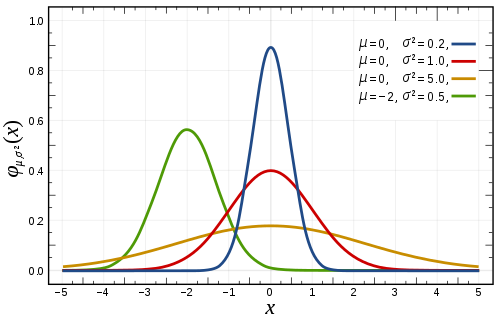
\includegraphics[width=0.46\textwidth]{img/normal}
      \caption{Quelle: Wikipedia}
\end{figure}
 \end{frame}




\begin{frame}
    \frametitle{Erwartungswert}
\framesubtitle{}
\begin{block}{Eigenschaften}
Sind $X,Y : \Omega \to \mathbb{R}^n$   reelle, integrierbare  Zufallsvariablen und $a,b \in \mathbb{R}$ konstant, so gilt:
\begin{align*}
& \mathbb{E}(a \cdot X + b \cdot Y) = a \cdot \mathbb{E}(X) + b \cdot \mathbb{E}(Y) \\
& X(x) \leq Y(x) \;  \forall x \in \Omega \Rightarrow \mathbb{E}(X) \leq \mathbb{E}(Y) \\
& X ,Y \text{ stoch. unabhängig} \Rightarrow   \mathbb{E}(X \cdot Y) =  \mathbb{E}(X) \cdot  \mathbb{E}(Y) \\
& \mathbb{E} (1_A) = P (A)
\end{align*}
\end{block}
 \end{frame}


\begin{frame}
    \frametitle{Erwartungswert}
\framesubtitle{}
\begin{block}{Markov Ungleichung}
Sei $Y : \Omega \to \mathbb{R}$  eine  reelle, integrierbare  Zufallsvariable und $f : [0, \infty) \to [0, \infty)$ monoton wachsend.
Dann gilt für alle $\epsilon > 0$ mit $f(\epsilon) > 0$
\begin{align*}
P (|Y |  \geq \epsilon) \leq \frac{\mathbb{E} (f \circ |Y|)}{f(\epsilon)}
\end{align*}
\end{block}
\begin{block}{Beweis}
Da $f(\epsilon) 1_{\{ |Y| \geq  \epsilon \} } \leq f \circ |Y|$ folgt
\begin{align*}
f(\epsilon) P(|Y| \geq \epsilon) = & f(\epsilon) \mathbb{E}(1_{\{ |Y| \geq  \epsilon \} }) = \mathbb{E}( f(\epsilon) 1_{\{ |Y| \geq  \epsilon \} }) \\
\leq & \mathbb{E}( f \circ |Y|)
\end{align*}
\end{block}
 \end{frame}


\begin{frame}
    \frametitle{Erwartungswert}
\framesubtitle{}
\begin{block}{Varianz}
Für eine reelle Zufallsvariable ist die Varianz definiert durch
$$ \mathbb{V} (X) :=  \mathbb{E}( (X - \mathbb{E}(X))^2) \; .$$
\end{block}
\begin{block}{Verschiebungssatz}

\begin{align*}
 \mathbb{V}(X) & = \mathbb{E}(X^2 - 2X \mathbb{E}(X) + \mathbb{E}(X)^2) = \mathbb{E}(X^2) - 2 \mathbb{E}(X)^2 +  \mathbb{E}(X)^2 \\
& =  \mathbb{E}(X^2) -  \mathbb{E}(X)^2 \\
\end{align*}
\end{block}
 \end{frame}


\begin{frame}
    \frametitle{Erwartungswert}
\framesubtitle{}
\begin{block}{Beispiel}
Sei $X \sim \mathcal{N}(\mu, \sigma^2)$.
\begin{align*}
&\mathbb{V} (X) =  \frac{1}{\sqrt{2 \pi}} \int_{- \infty}^{\infty} x^2 e^{- \frac{x^2}{2}} \; dx =   \frac{1}{\sqrt{2 \pi}} \int_{- \infty}^{\infty} x (xe^{- \frac{x^2}{2}}) \; dx \\
& =  \frac{1}{\sqrt{2 \pi}} \biggl (\biggl [ x (e^{- \frac{x^2}{2}}) \biggr]_{- \infty}^{\infty}   - \int_{- \infty}^{\infty}  - e^{- \frac{x^2}{2}} \; dx  \biggr) = 0 + 1 = 1\\
\end{align*}
\href{https://de.wikipedia.org/wiki/Partielle_Integration}{LINK: Partielle Integration}. Mit "Verschiebungstrick"
$\Rightarrow \mathbb{V}(X) = \sigma^2$.
\end{block}
 \end{frame}


\begin{frame}
    \frametitle{Erwartungswert}
\framesubtitle{}
\begin{block}{Tschebyscheff-Ungleichung}
Für eine reelle, integrierbare und quadratintegrierbare  Zufallsvariable $Y : \Omega \to \mathbb{R}$  gilt:
\begin{align*}
P (|Y  - \mathbb{E} (Y)|  \geq \epsilon) \leq \frac{\mathbb{V} (Y)}{ \epsilon^2} 
\end{align*}
\end{block}
\begin{block}{Beweis}
Folgt direkt aus der Markov-Ungleichung mit $Y' = Y -\mathbb{E}(Y)$ und $f(x) = x^2$
\end{block}
 \end{frame}


\begin{frame}
    \frametitle{Highlight}
\framesubtitle{}
\begin{figure}[htp]
      \centering
    
\includegraphics[width=0.9\textwidth]{img/firework}
\end{figure}
 \end{frame}


\begin{frame}
    \frametitle{Erwartungswert}
\framesubtitle{}
\begin{block}{Schwaches Gesetz der großen Zahlen}
Seien $X_i : \Omega \to \mathbb{R}$ unabhängige, reelle Zufallsvariablen (uid, iid(englisch)) mit $\mathbb{E}(X_i) = \mu < \infty$ und $\mathbb{V}(X_i) = \sigma < \infty$, dann gilt
\begin{align*}
P \bigl  ( \bigl | \frac{1}{n} \sum_{i=1}^{n} X_i - \mu \bigr |  \geq \epsilon \bigr) \leq \frac{\sigma}{ n \cdot \epsilon^2} \; \; \underset{n \to \infty}{\longrightarrow} 0
\end{align*}
(stochastische Konvergenz). 
\end{block}
 \end{frame}


\begin{frame}
    \frametitle{Erwartungswert}
\framesubtitle{}
\begin{block}{Beweis}
Mit $Y_n =  \frac{1}{n} \sum_{i=1}^{n}  X_i - \mu$ ist $\mathbb{E}(Y_n) =  \frac{1}{n} \sum_{i=1}^{n} \mathbb{E}( X_i - \mu) = 0$ und 
$\mathbb{V}(Y_n) =  \frac{1}{n^2} \sum_{i=1}^{n} \mathbb{V}( X_i ) = \frac{\sigma}{n}$. Aus der Tschebyscheff-Ungleichung folgt die Behauptung.
\end{block}
 \end{frame}


\begin{frame}
    \frametitle{Erwartungswert}
\framesubtitle{}

\begin{figure}[htp]
      \centering
    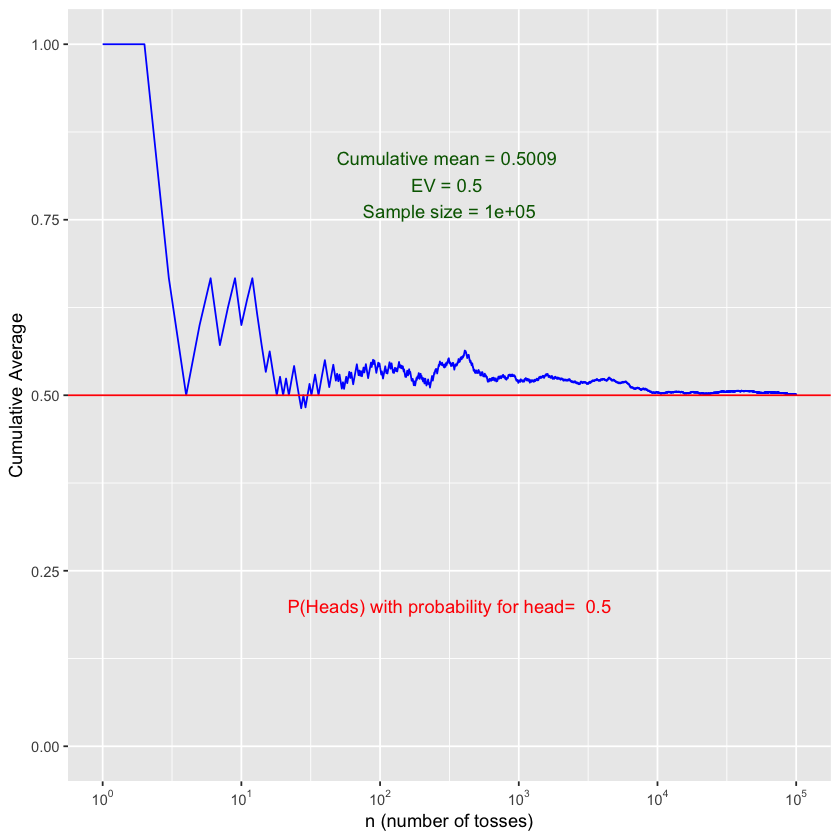
\includegraphics[width=0.86\textwidth]{img/sgdz}
      \caption{Quelle: Wikipedia}
\end{figure}
 \end{frame}



\end{document}

